\documentclass[18pt]{article}
\usepackage[utf8]{inputenc}
\usepackage[T1]{fontenc}
\usepackage{ragged2e}
\usepackage{caladea}
\usepackage{graphicx}
\usepackage{longtable}
\usepackage{wrapfig}
\usepackage{rotating}
\usepackage{epigraph}
\usepackage[normalem]{ulem}
\usepackage{hyperref}
\usepackage{amsmath}
\usepackage{amssymb}
\usepackage{capt-of}
\usepackage{hyperref}
\usepackage{fancyhdr}

\title{
 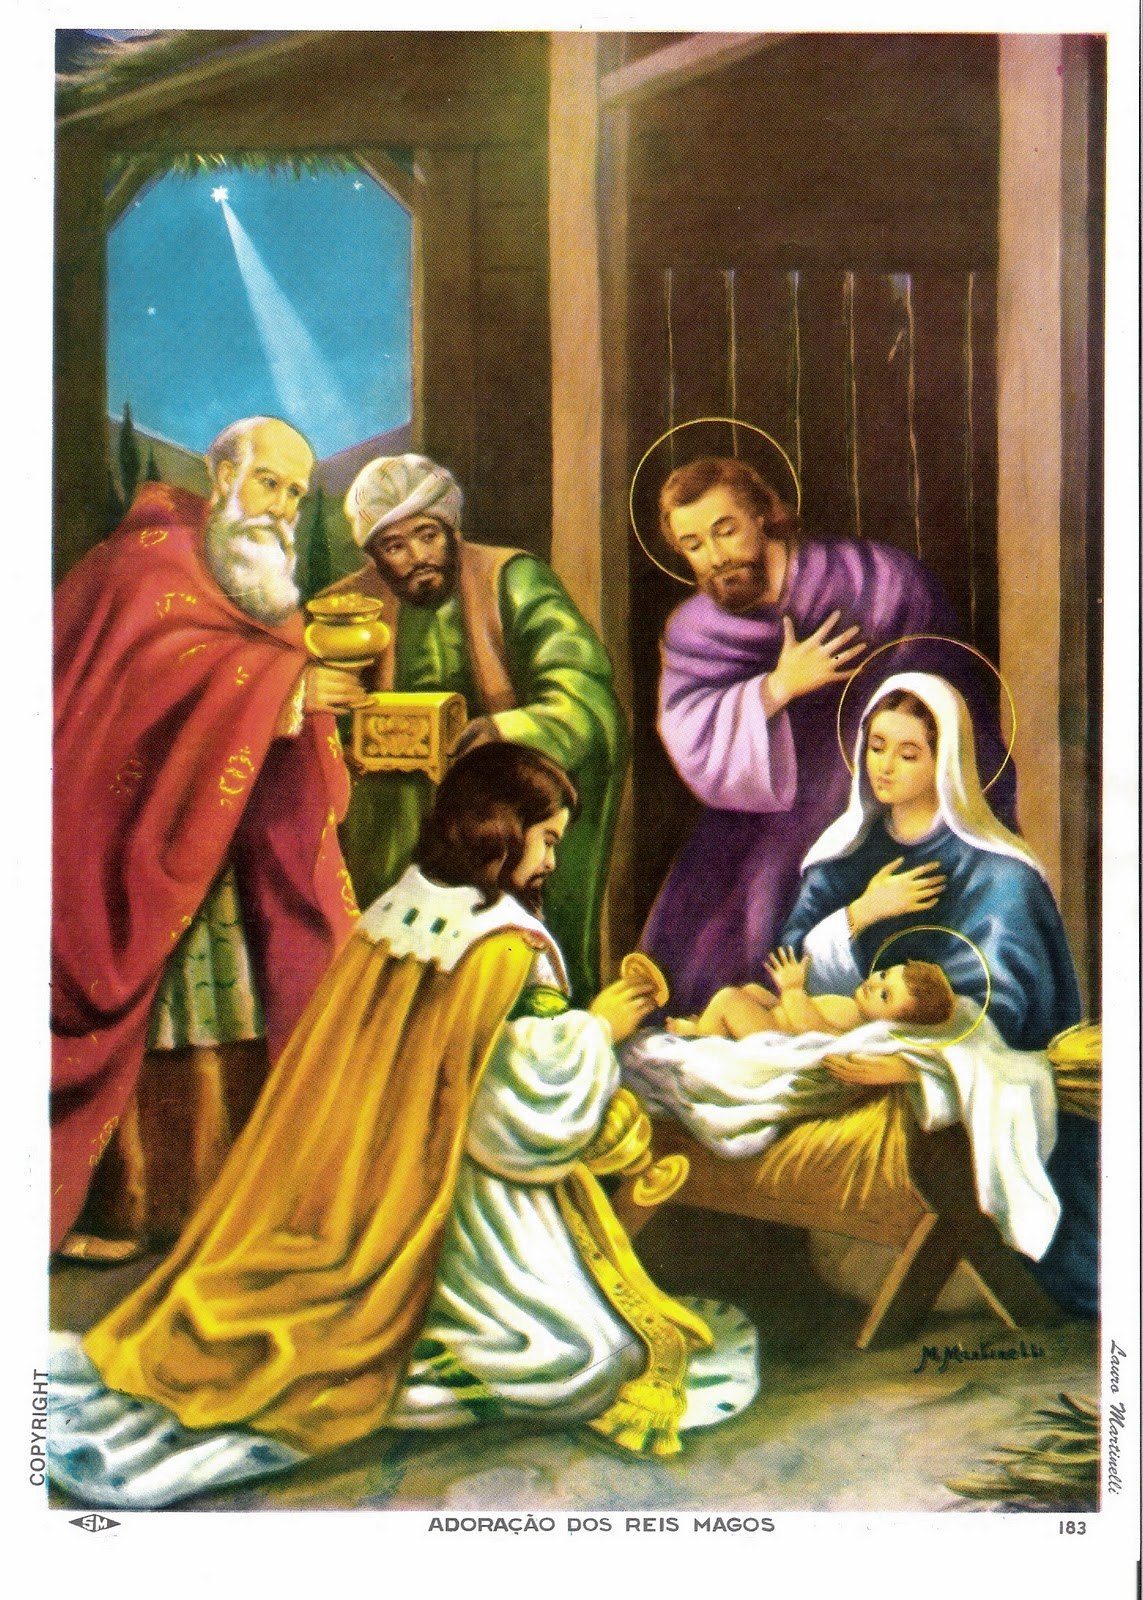
\includegraphics[scale=0.25, trim={10cm, 0, 10cm, 0}]{./assets/imagem.jpg}
  \par
   NOVENA AOS SANTOS REIS MAGOS}
\author{Garamog, Nina Freitas}
\date{Início da Novena: 28/12 - Data Litúrgica: 06/01 }

% Comando para fazer "Sumário" não aparecer no Sumário.
\renewcommand{\contentsname}{Sumário}
\begin{document}
\maketitle

\thispagestyle{empty} %zera a primeira página


\pagestyle{fancy}
\fancyhf{} % clear existing header/footer entries
\fancyfoot[LO, CE]{
  
\includegraphics[scale=0.2]{./assets/cross.png} Santos Reis Magos, rogai por nós!
}
% Place Page X of Y on the right-hand
% side of the footer
\fancyfoot[R]{\thepage}

\newpage

\tableofcontents

\centering
\vfill
Visite-nos no Telegram: \url{https://t.me/CotidieNovena}
\newpage

\newpage

%%%%%%%%%%%%%%%%%%%%%%%%%%%%%%%%%%%%% Orações  %%%%%%%%%%%%%%%%%%%%%%%%%%%%%%%%%%%%%%%%%%%

\section{Orações}\label{sec:Orações} % (fold)

\subsection{1° Dia}

“Vê, a noite cobre a Terra, e a escuridão, os povos, mas sobre ti levanta-se o Senhor, e Sua glória te ilumina.” (Isaías 60,2). 

Ó Santos Magos, que vivestes em contínua espera da Estrela de Jacó, que viria a anunciar o Nascimento do verdadeiro Sol de Justiça, obtende-nos a graça de viver sempre na esperança de ver surgir sobre nós o dia da verdade, a beatitude do Paraíso. 



\textbf{\nameref{sub:oracao_final}}


\subsection{2° Dia}

“Levanta os olhos e olha à tua volta: todos se reúnem para vir a ti” (Isaías 60,4).  

Ó Santos Magos, que ao primeiro brilho da Estrela milagrosa abandonastes os vossos Países para ir à procura do Rei dos Judeus recém-nascido, obtende-nos a graça de corresponder prontamente, como vós, a todas as divinas aspirações. 


\textbf{\nameref{sub:oracao_final}}


\subsection{3° Dia}

“Os teus filhos chegam de longe, e tuas filhas são transportadas nos braços.” 

Ó Santos Magos, que não temestes os rigores das estações nem os desconfortos da viagem para conseguirem encontrar o nascido Messias, obtende-nos a graça de não nos deixar jamais esmorecer diante das dificuldades que se encontram no caminho da Salvação.


\textbf{\nameref{sub:oracao_final}}


\subsection{4° Dia}

“As nações caminharão para à tua luz, e os reis, para o brilho de tua aurora.” (Isaías 60,3).

Ó Santos Magos, que, abandonados pela Estrela na cidade de Jerusalém, recorrestes com humildade e sem humano respeito a quem pudesse vos dar certa notícia do lugar onde se encontrava o objeto de vossas buscas, obtende-nos a graça de, em todas as dúvidas, em todas as perplexidades, nós recorrermos humildemente, e fielmente sigamos os conselhos dos nossos superiores que representam sobre a Terra a própria pessoa de Deus. 


\textbf{\nameref{sub:oracao_final}}


\subsection{5° Dia}

“Essa visão te tornará radiante; teu coração palpitará e se dilatará” (Isaías, 60,5).

Ó Santos Magos, que, contra toda vossa esperança, fostes novamente consolados pela Estrela que reapareceu para vos servir de guia, obtende-nos do Senhor a graça de, permanecendo a Ele fiéis em todas as aflições, mereçamos ser consolados por Sua graça, no tempo, e por Sua glória, na eternidade. 


\textbf{\nameref{sub:oracao_final}}



\subsection{6° Dia}

“... porque para ti afluirão as riquezas do mar, e a ti virão os tesouros das nações.” (Isaías, 60,5).

Ó Santos Magos, que, entrando cheios de fé no estábulo de Belém, prostrados à terra, adorastes o nascido Rei dos Judeus, ainda que não fosse cercado que pelos indícios de pobreza e fragilidade, obtende-nos do Senhor a graça de reavivar sempre a nossa Fé quando entrarmos em Sua casa, a fim lá habitarmos com aquele respeito que é devido à grandeza de sua Majestade. 


\textbf{\nameref{sub:oracao_final}}



\subsection{7° Dia}

“Serás invadida por uma multidão de camelos, pelos dromedários de Madiã e de Efá; virão todos de Sabá, trazendo Ouro e Incenso, e proclamando os louvores do Senhor.” (Isaías, 60,6).

Ó Santos Magos, que, oferecendo a Jesus Cristo Ouro, Incenso e Mirra, O reconhecestes concordes como Rei, como Deus e como Homem, obtende-nos do Senhor a graça de não nos apresentarmos nunca de mãos vazias diante d’Ele, mas que Lhe ofereçamos o Ouro da caridade, o Incenso da adoração e a Mirra da penitência, visto que sem essas virtudes é impossível encontrar o Seu agrado. 


\textbf{\nameref{sub:oracao_final}}


\subsection{8° Dia}

“Porque a nação ou o reino que recusar servir-te perecerá, e sua terra será devastada.” (Isaías, 60,12).

Ó Santos Magos, que, avisados por um Anjo para não voltar a Herodes, vos encaminhastes logo por outra estrada à vossa Pátria, obtende-nos do Senhor a graça de, após termos nos reconciliado com Ele nos Santos Sacramentos, vivamos apartados de tudo aquilo que poderia ser para nós ocasião de novos pecados.


\textbf{\nameref{sub:oracao_final}}


\subsection{9° Dia}

“Levanta-te, revista-te de luz, eis a tua Luz! A glória do Senhor se levanta sobre ti.” (Isaías, 60,1)

Ó Santos Magos, que, chamados os primeiros entre os Gentios ao conhecimento de Jesus Cristo, perseverastes até à morte na vossa profissão de Sua Fé, obtende-nos do Senhor a graça de sempre viver em conformidade com as promessas por Ele feitas no Santo Batismo, ou seja, de renunciar constantemente ao mundo e às suas pompas, à carne e às suas tentações, ao demônio e às suas sugestões, a fim de nos merecer como vós a visão beatifica daquele Deus que forma aqui na Terra o objeto de nossa Fé 


\textbf{\nameref{sub:oracao_final}}

\subsection{Oração Final}\label{subsec:OraçãoFinal} % (fold)

\textbf{Pai Nosso, Ave Maria, Glória ao Pai.}

\subsection*{Créditos:}
\href{https://catholicnovenaprayer.com/novena-prayer-to-pope-st-sylvester-i/}{Catholic Novena Prayer}


\subsection{Oração Final}\label{sub:oracao_final} % (fold)

Ó perfeitíssimos adoradores do recém-nascido Messias,
Santos Magos, verdadeiros modelos do cristão de coragem, 
Vós, que nada vos desanimou da árdua jornada. 
E que, prontamente, ao sinal da estrela, 
Seguistes as divinas aspirações, 
Obtende-nos do Senhor a graça de, à vossa imitação, 
Sempre ir a Jesus Cristo 
E de adorá-lO com viva Fé 
Quando entrarmos em Sua Casa. 

Fazei que Lhe ofereçamos continuamente
O Ouro da caridade, 
O Incenso da oração, 
A Mirra da penitência, 
E não declinemos jamais da estrada da santidade, 
Que Jesus nos ensinou tão bem com Seu próprio exemplo, 
Antes mesmo do que com Seus ensinamentos;

Fazei, ó Santos Magos, que possamos merecer do Divino Redentor
As Suas eleitas bênçãos aqui na Terra
E a imerecida posse, depois, da glória eterna. Amém. 

\textbf{Glória ao Pai (3 vezes)}

Sancti Reges Magi, orate pro nobis. 

Em nome do Pai, do Filho, do Espírito Santo. Amém.




\end{document}
